\chapter{Diseño y desarrollo\label{sec:disenhoYDesarrollo}}

%\textbf{Rápida intro.}

%En esta sección se presentan los resultados de las fases de análisis de requisitos, diseño y desarrollo realizadas para el proyecto.
%
%Al ser un proyecto asociado a una investigación que se ha desarrollado en varias fases, se consideró que una mejor metodología que se podía utilizar era una basada en el modelo en espiral descrito en \cite{Boehm86} . A pesar de que la metodología presenta varias iteraciones en cada fase, aquí se presentan los resultados agrupados.

En este capítulo se presentan las partes más relevantes de las fases de análisis, diseño y desarrollo del proyecto. Primero, se detallarán todos los requisitos, funcionales y no funcionales, que se han identificado. A continuación, las ideas principales detrás del diseño implementado y para terminar, se detalla aquello más relevantes de la fase de desarrollo.

Como este proyecto nació asociado a una investigación, no se ha utilizado una metodología en cascada clásica, sino un modelo en espiral, partiendo del descrito en \cite{Boehm86}. A pesar de que el modelo describe varias iteraciones, en esta sección se presentan agrupados los resultados finales a los que se han llegado entre todas las iteraciones, para facilitar su lectura.

%TODO: Demostrar todo el dominio que pueda sobre cuestiones de la carrera.

\section{Análisis de requisitos}

Los requisitos aquí detallados son el fruto de un análisis a priori sobre qué necesidades tenía que cubrir el sistema más carencias que se han detectado al ser utilizado en entorno reales y que se han ido añadiendo. Algunas de las mejoras posibles se han detectado en la última iteración realizada, aún no están implementadas y en consecuencia, aquí no se recogen. Aún así, están recogidas en el apéndice \ref{apen:analisis de requisitos}. 

\subsection{Análisis funcional}

\begin{rf0}

	\item \textbf{Gestión de usuarios.}
			\begin{rf0*}
				\item El sistema deberá permitir crear cuentas de usuario. Las cuentas tendrán un nombre de usuario y contraseña que identifiquen a cada usuario.
				\item Cada cuenta de usuario tendrá un rol en cada asignatura en la que participe. Podrá ser un rol docente o rol estudiante. Dependiendo del rol que tenga, la cuenta podrá acceder a más o menos funcionalidad en cada sección del sistema, como se detalla más adelante.
				\item El equipo docente de cada asignatura determinará qué alumnos pertenecen a sus grupos.
			\end{rf0*} 

	\item \textbf{Creación y gestión de materias.}  \textit{Rol docente.} 
			\begin{rf0*}
				\item Dentro de su asignatura, el docente podrá crear tantas materias como necesite. Cuando cree una materia, deberá establecer un título, el número de niveles en los que se clasificarán las preguntas y el número de respuestas que tendrá cada una.
				\item Una vez creada una materia, el docente podrá modificar su configuración. Podrá cambiar el título en cualquier caso, pero solo podrá cambiar el número de niveles y el número de respuestas cuando no haya preguntas asociadas a la materia o cuando el número aumente. Para disminuir alguno de los dos valores, deberá borrar antes todas las preguntas asociadas a la materia.
			\end{rf0*}

	\item \textbf{Creación y gestión de preguntas y respuestas.}  \textit{Rol docente.} 
		\begin{rf0*}
			\item Existiendo al menos una materia, los docentes podrán crear preguntas y respuestas asociadas a dicha materia.
			\item Cuando se cree una pregunta nueva, deberá indicarse la materia a la que pertenece (que deberá haber sido creada previamente), el nivel, el enunciado, la respuesta correcta y el resto de respuestas. El número de respuestas que deberá escribir vendrá condicionado por el valor establecido en la materia relativa.
			\item Opcionalmente, se podrá asociar ficheros multimedia a las preguntas. Se pueden asociar imágenes o audio tanto al enunciado como a cada una de las respuestas. Si se desea asociar un fichero multimedia, deberá especificarse el nombre del fichero.
			\item Opcionalmente, se podrá establecer un mensaje de feecback asociado a la pregunta.
			\item Una vez creada una pregunta, el docente podrá modificar cualquier atributo o borrar dicha pregunta. En ambos casos, se mantendrá una copia en la base de datos de la antigua pregunta para que los alumnos no vean alterados sus cuestionarios una vez realizados.
		\end{rf0*}
	
	\item \textbf{Subida y gestión de ficheros multimedia.}  \textit{Rol docente.} 
		\begin{rf0*}
			\item Existiendo al menos una materia, los docentes podrán subir un fichero de audio (en formato mp3) o imagen (con extensión gif, png, jpeg o jpg) y asociarlo a dicha materia para utilizarlos después en alguna pregunta de la materia.
			\item Se podrá consultar un listado de todos los ficheros multimedia ya subidos a una materia, que mostrará el nombre de cada fichero además de mostrar la imagen o permitir reproducir el audio.
			\item Se podrá actualizar un fichero subiendo otro al servidor con el mismo nombre.
		\end{rf0*}

	\item \textbf{Rol docente:} Creación y gestión de cuestionarios.
		\begin{rf0*}
			\item Existiendo al menos una materia y preguntas suficientes en cada nivel, el profesor podrá crear un cuestionario. Al hacerlo deberá definir un nombre, si el cuestionario será visible a los alumnos, la materia que se usará como banco de preguntas, el número de preguntas que deberán contestarse en cada intento, el tiempo máximo, si el examen acepta respuestas con duda y cómo deberán mostrarse el resultado a los alumnos.
			\item Una vez creado un cuestionario, el docente podrá eliminar el cuestionario. Esto no afectará, en ningún caso, a la información almacenada sobre los cuestionarios ya respondidos por alumnos.
			\item Los docentes podrán acceder a un listado de todos los cuestionarios ya creados.
		\end{rf0*}
		
	\item \textbf{Realización de cuestionarios.} 
		\begin{rf0*}
			\item Una vez creado un cuestionario por un profesor, y si está marcado como visible, los alumnos podrán acceder a él.
			\item Una vez que un estudiante acceda a un cuestionario, se le irán mostrando preguntas que deberá ir contestando. Las preguntas se mostrarán en función de las respuestas previas y los niveles establecidos por el profesor.
			\item Si las preguntas van asociadas a ficheros multimedia, estos se mostrarán al estudiante mientras responde. Si aceptan la opción de responder con duda, el alumno tendrá a su disposición un método de establecer que ha respondido con duda.
			\item Para cada pregunta que el alumno responda, quedará almacenado en el sistema a qué cuestionario pertenece, cuando se responde, qué pregunta se ha formulado y cuál ha sido la respuesta elegida. Si hubiera opción de duda, también se mostrará si se ha dudado o no al responder.
		\end{rf0*}
	
	\item  \textbf{Visualización de resultados.}
		\begin{rf0*}
			\item Si el profesor ha establecido que los resultados se muestren al terminar el examen, se mostrará la nota final, todas las preguntas, junto con cuál ha sido la respuesta del alumno para cada pregunta y si esta ha sido correcta. El profesor también puede elegir que solo se muestre la nota, o ninguna información.
			\item Cuando una pregunta tenga una cadena de feedback asociada, se mostrará a los alumnos después de que respondan, junto con si la respuesta ha sido correcta o no.\label{RF:feedback}
			\item \textbf{Rol docente:} Los docentes podrán acceder a un listado con todos los intentos que han realizado cada alumno a cada cuestionario que hayan creado. Para cada cuestionario, podrán ver el detalle de cada uno, es decir, qué preguntas se respondieron, cuál fue la respuestas, si era correcta y el instante en el que se respondió.
		\end{rf0*}

	\item  \textbf{Análisis de resultados.} \textit{Rol docente.}
		\begin{rf0*}
			\item El sistema implementará sistemas automáticos que ayuden al equipo docente a detectar preguntas conflictivas, es decir, aquellas donde el número de fallos sea inusualmente elevado, para que los docentes puedan analizar y corregir los defectos asociados a dichas preguntas.
		\end{rf0*}
\end{rf0}


\subsection{Análisis no funcional}

\begin{rnf0}
	\item \textbf{Interfaz y usabilidad.}
		\begin{rnf0*}
			\item La interfaz que el sistema mostrará al estudiante debe ser intuitiva y fácil de usar para todas las edades. Estudiantes alfabetizados deben ser capaces de elegir un cuestionario y completarlo sin asistencia externa. Una clase de niños que aún no sepan leer debe ser capaz de completar un cuestionario sin asistencia del profesor, después de que este les haya configurado el ordenador para que el cuestionario elegido empiece.\label{RNFusabilidad}
			\item La interfaz para el equipo docente deberá ser fácil de aprender para profesores con o sin conocimientos informáticos avanzados. 
			\item Atendiendo a la diversidad de dispositivos con los que los usuarios trabajan, el sistema debe ser capaz de utilizarse en todos los tamaños de pantalla y para ser utilizado con teclado y ratón o pantalla táctil.
		\end{rnf0*}
	\item \textbf{Seguridad.}
		\begin{rnf0*}
			\item Debido al carácter secreto de gran parte del contenido creado por los profesores, el sistema deberá garantizar la no accesibilidad de ese contenido a usuarios no autorizados.
			\item Todo usuario que acceda al sistema debe autentificarse previamente a través de un usuario/contraseña, para asegurar la autoría de las respuestas de los cuestionarios.
			\item La autentificación de los usuarios debe ser segura. En concreto, el sistema no almacenará las contraseñas en la base de datos en texto plano. Deberá utilizar un método que garantice que la contraseña no sea conocida aunque se acceda a la base de datos.
		\end{rnf0*}
	\item \textbf{Modularidad.}
		\begin{rnf0*}
			\item El diseño realizado tiene que permitir que el modelo de evaluación sea fácilmente modificable, es decir, que las modificaciones que se realicen en el modelo de evaluación involucren exclusivamente a una región claramente delimitada del código repartida exclusivamente en un fichero. \label{RNF:mofularidad}
		\end{rnf0*}
	\item \textbf{Rendimientos.}
		\begin{rnf0*}
			\item El sistema debe permitir que, al menos, 50 usuarios realicen a la vez un mismo cuestionario.
		\end{rnf0*}
\end{rnf0}


%\textbf{¿Detallar un análisis funcional? Sí}

\section{Diseño}

Los sistemas adaptativos pueden abstraerse como una serie de módulos como los descritos en la figura \ref{fig:diagrama_disenno}. 

\begin{figure}[htp!]
	\centering
	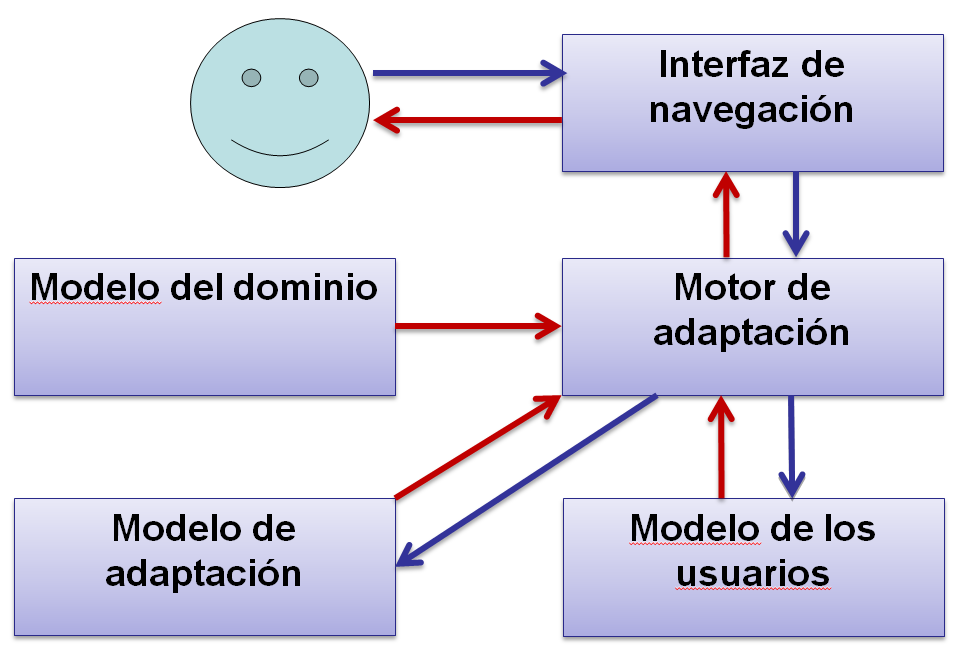
\includegraphics[width=0.75\textwidth,clip=true]{diagrama_disenno}
	\caption{División en módulos de un sistema adaptativo}
	\label{fig:diagrama_disenno}
\end{figure}

El usuario (representado arriba a la izquierda) interacciona con el sistema a través de una interfaz de navegación que representa el estado del motor de adaptación, componente que articula al resto de módulos. El modelo del dominio, de adaptación y el modelo de los usuarios son las herramientas de las que el motor de adaptación obtiene la información que le permite dar una respuesta adecuada a cada situación. Mientras que el modelo del dominio es fijo, en el sentido de que permanece estable durante la vida del mismo, el modelo de adaptación y el modelo de los usuarios van sufriendo variaciones, en función de la entrada que produzcan los usuarios.

Durante las siguientes secciones se dará una descripción más detallada de los módulos.

\subsection{Interfaz de navegación}

La interfaz de navegación es la parte del sistema encargada de permitir la interacción entre el sistema y el usuario. Debe representar ante el usuario la información del sistema que este deba conocer, además de recibir la entrada que el usuario genere para que el motor de adaptación pueda incorporarla.

En el diseño seguido para este trabajo se decidió utilizar las tecnologías web como base sobre la que construir, por lo que las funciones de la interfaz de navegación recaen principalmente en el navegador web del usuario. Aún así, el sistema debe crear y, sobre todo, adaptar los ficheros html que envía al navegador del cliente. Para ello se han utilizado las tecnologías web estándar: HTML, Javascript, CSS y PHP. Más información sobre las tecnologías utilizadas en \ref{sec:tecnologias}.

\subsection{Modelo de los usuarios}

%\textbf{Profesor y estudiante}

El sistema tiene dos roles de usuarios claramente diferenciados: rol docente y rol estudiante. Las necesidades que tienen ambos roles respecto de la aplicación, son radicalmente distintas. Mientras que a los docentes se les debe mostrar herramientas para la creación y gestión de cuestionarios, motorización de resultados y recuperación de exámenes, los estudiantes deben acceder a la ejecución de los cuestionarios, a cierta retroalimentación y a sus resultados.

En ninguno de los dos roles podemos presuponer conocimientos informáticos avanzados, como se recoge en \ref{RNFusabilidad}. Además, el sistema debe ser fácil de usar para docentes y estudiantes de todas las etapas educativas, desde la primera infancia hasta la edad adulta. Al ser una aplicación potencialmente disponible a niños y niñas muy jóvenes, tampoco podemos presuponer que el estudiante sepa leer, debiendo dotar en consecuencia al rol del docente la habilidad de incluir ficheros multimedia con los que suplir dicha carencia.

\subsection{Modelo del dominio}

La aplicación pretende ser una ayuda al aprendizaje y por lo tanto, su dominio es la actividad educativa. Más concretamente, aquellas actividades relacionadas con comprobar, por parte del propio estudiante o de un docente, si el alumno ha adquirido correctamente ciertos conocimientos. Para ello, a grandes rasgos, el equipo docente de una asignatura creará una serie de preguntas y respuestas, agrupadas por su contenido en materias, que utilizará para crear cuestionarios a los que los estudiantes tendrán acceso. Del resultado de dichos cuestionarios, tanto el estudiante como los docentes podrán conocer cómo están realizando su actividad y realizar los cambios que fueran necesarios.

La asignatura es la primera división que se utiliza normalmente en los entornos educativos. Un docente se encarga de unas asignaturas en concreto y los estudiantes van explorando el conocimiento por asignaturas. Así, cada asignatura tiene asociados un listado de usuarios, algunos comos docentes y otros como estudiantes. Es importante notar que un usuario podría ser docente en una asignatura pero estudiante en otra, por lo que el rol es un atributo de la unión usuario y asignatura, y no solo del usuario.

Dentro de cada asignatura, existen una serie de materias, que son las entidades que clasifican los conocimientos por similitud dentro de una asignatura. El concepto de materia en este modelo se utiliza para representar los conceptos del lenguaje común de \emph{temas} o \emph{partes} en los que se divide una asignatura. Dentro de cada materia existe un conjunto de preguntas, ordenadas por un nivel de relevancia.

La división de las preguntas en niveles de relevancia es una de las características del modelo propuesto. Con ello se busca facilitar que el estudiante adquiera los conocimientos en el orden más adecuado, asegurando que no se enfrenta a conceptos que dependen de otros hasta que domina los conceptos base. Esta división también ayuda a evitar que un estudiante obtenga una buena calificación en un examen porque haya aprendido a realizar los ejercicios, pero aún así carezca de entendimiento sobre los conceptos básicos. Una discusión más detallada sobre el sistema de clasificación de las preguntas en niveles puede encontrarse en el apéndice \ref{apend:preguntas en niveles}.

Cada pregunta lleva asociada una serie de respuestas y solo una es la válida. Tanto las preguntas como las respuestas llevan asociadas mucha información, como el enunciado, imágenes opcionales\ldots

Una vez escrito un número suficiente de preguntas, el equipo docente puede crear cuestionarios. Las cuestionarios pueden ser de autoevaluación para los alumnos o de evaluación clásica, aunque para el sistema son casos idénticos.

%\textbf{Estructura de la BD}

\subsection{Modelo de adaptación\label{sec:modelo adapatacion}}

El sistema contempla dos tipos de adaptación. Primero, tenemos la adaptación de navegación, que es aquella que busca guiar al usuario por el sistema, facilitando su uso. En nuestro caso, la navegación del estudiante es sencilla, por lo que no aplica. Donde sí que es necesario este tipo de adaptación es en el área del docente. A la hora de crear las materias, las preguntas y los cuestionarios existe un orden de trabajo más sencillo que otros y el sistema deberá guiar al usuario por ese recorrido utilizando elementos variables de la interfaz.

%\begin{figure}[htp!]
%	\centering
%	\includegraphics[width=0.5\textwidth,clip=true]{adaptacion_navegacion}
%	\caption{}
%	\label{fig:adaptacion de navegacion}
%\end{figure}

El otro tipo de adaptación, la adaptación del contenido, es la más relevante para el sistema. Al igual que la de navegación afecta principalmente al docente, la de contenido afecta sobre todo al estudiante. Las preguntas a las que un estudiante se enfrenta en un cuestionario depende de las respuestas que haya dado a las anteriores.

En concreto, cuando un docente crea un cuestionario establece dos parámetros, $N_l$, que es el número de niveles en los que una pregunta se puede clasificar y $N_v$, que es el número de preguntas que debe responder cada alumno en cada intento del cuestionario. Todos los estudiantes empiezan respondiendo a preguntas del primer nivel y solo se enfrentarán a preguntas de niveles más avanzados cuando hayan respondido correctamente a suficientes preguntas. En concreto, a $\frac{N_v}{N_l}$ preguntas.

\begin{figure}[htp!]
	\centering
	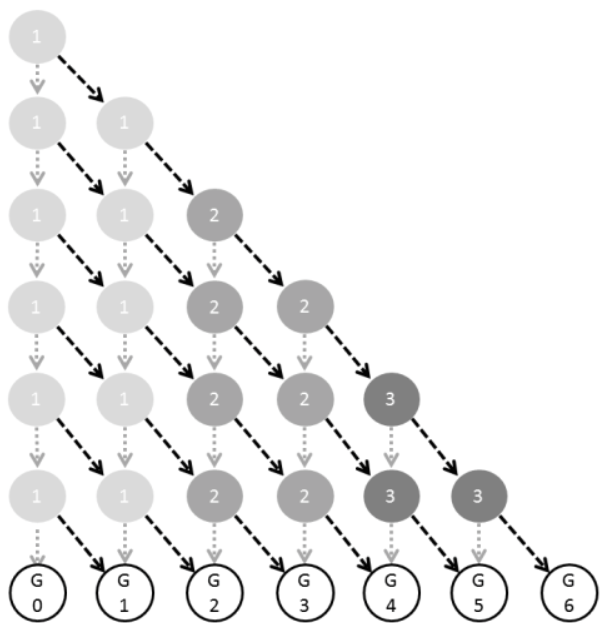
\includegraphics[width=0.5\textwidth,clip=true]{modelo_adaptacion}
	\caption[Modelo de adpatación]{Diagrama que representa todos los posibles recorridos para un cuestionario con $N_l = 3$ y $N_v = 6$. Todos los alumnos entran por la pregunta de la esquina superior izquierda. El número dentro de las circunferencias representa la dificultad de la pregunta. Cuando un alumno responde, toma el camino de la flecha oscura cuando acierta y de la flecha clara cuando falla. La última fila del diagrama representa las posibles notas que un estudiante puede sacar, ordenadas de menor a mayor de izquierda a derecha.}
	\label{fig:modelo de adaptacion}
\end{figure}

La elección de la siguiente pregunta dentro de un mismo nivel se hace de forma aleatoria, asegurando en todo momento que no haya preguntas repetidas dentro del mismo cuestionario. Cuando el alumno sube de nivel, ya solo responde a preguntas de ese nuevo nivel. Como el número de preguntas está limitado, es posible que un estudiante no llegue a responder preguntas de todos los niveles o incluso puede que solo responda preguntas del primer nivel. Una vez que se ha subido de nivel, no se puede bajar, aunque cada vez que se repita el cuestionario se volverá al primer nivel.

Que la respuesta de una pregunta condicione la siguiente pregunta obliga a que el estudiante responda a cada pregunta, a diferencia de los cuestionarios clásicos, donde una pregunta puede dejarse sin respuesta y continuar con la siguiente. Para solucionar esta diferencia el equipo docente puede establecer que exista una opción adicional de respuesta que indique que el alumno no conoce la respuesta. Si marca está opción, el sistema la tratará como respuesta incorrecta a la hora de seleccionar la siguiente pregunta. Así mismo, la aplicación da al docente la opción de mostrar una casilla que especifique que el alumno ha respondido sin estar seguro de que sea la respuesta correcta. Más información sobre el modelo del examen, en concreto sobre el sistema de calificación, puede encontrarse en el apéndice \ref{apen:como se ponen las notas}

Así mismo, el docente puede decidir que los estudiantes reciban feedback al responder una pregunta o no, como se describe en \ref{RF:feedback}.

%\textbf{Exámenes con distintos niveles y cómo se pasa de uno a otro. Hablar también del feedback o del no lo sé}

\subsection{Motor de adaptación}

El reto del motor de adaptación está en que tiene que ser bastante flexible, para poder permitir cambios en alguno de los modelos sin que eso requiera cambios en el resto. Este desarrollo se ha realizado asociado a una investigación que tenía entre sus objetivos el desarrollo de nuevos modelos de evaluación, que en nuestro caso de traduce en nuevos modelos de adaptación, por lo que al menos sabemos que ese módulo muy posiblemente cambiará. Siendo así, y como ya se recoge en \ref{RNF:modularidad}, en este diseño es de especial importancia que modificar el modelo de adaptación del examen sea sencillo. Para ello, los modelos de usuario y el modelo del dominio se pensaron de la forma más abstracta posible, además de dejar muy delimitado el código asociado al modelo de adaptación, además de hacerlo depende lo mínimo posible de todo lo demás.

%\textbf{Rápidas notas sobre la aplicación en sí. O no.}


\section{Desarrollo: e-valUAM\label{sec:desarrollo}}

En esta sección se detalla cómo se han plasmado los requisitos y el diseño del proyecto en la plataforma online creada, \acrshort{e-valUAM}, tomando como referencia lo expuesto en las secciones anteriores del presente capítulo.

\subsection{Visión general}

\acrshort{e-valUAM} es el sistema web de creación y respuesta de cuestionarios para ayuda al aprendizaje en el que se ha plasmado este proyecto. Es un sistema que ha sido desarrollado para servir como herramienta de una investigación que viene existiendo desde los últimos tres años, tomando su forma definitiva especialmente en el último año. Para cada año académico se construyó un prototipo diferente que siempre fue una ampliación del prototipo anterior, siguiendo un modelo de desarrollo en espiral.

Además, esta sección está complementada por la información disponible en los apéndices \ref{apen:estructura proyecto} y \ref{apen:codigo}, que hacen referencia a cómo está estructurado el código del proyecto y las partes del código más relevantes, respectivamente.

Por último, y puesto que el sistema requiere de autentificación para poder ser explorado, se ha creado una cuenta a tal propósito cuyo nombre de usuario y contraseña son \textit{TFG}. El sistema está disponible en \url{http://sacha.ii.uam/e-valUAM} para acceder como alumno y en \url{http://sacha.ii.uam/e-valUAM/profesor} para acceder como profesor. La cuenta tiene permisos tanto de alumno como de profesor, por lo que se pueden explorar libremente todo el sistema.

\subsection{Tecnologías y lenguajes empleados\label{sec:tecnologias}}

Al ser un sistema web, los lenguajes principales son aquellos relacionados con las tecnologías web. En concreto, se ha utilizado HTML5, CSS3 y Javascript para la parte del cliente, mientras que en el servidor se ha utilizado PHP 5. Para el desarrollo de la interfaz de usuario se han utilizado las librerías de Bootstrap 3 y jQuery.

En el lado del servidor se ha utilizado una máquina alojada en la UAM, con sistema operativo Windows 7, servidor Apache 2.2 y como gestor de base de datos PostgreSQL 9.3.

Como editor de código se ha utilizado Sublime Text 3. Para el control de versiones git y como repositorio central, Github.


\subsection{Base de datos}

Para este proyecto se eligió una base de datos relacional al existir una clara estructura en los datos que convenía respetar. En la figura \ref{fig:base de datos} se puede ver el diagrama entidad-relación.

\begin{figure}[htp!]
	\centering
	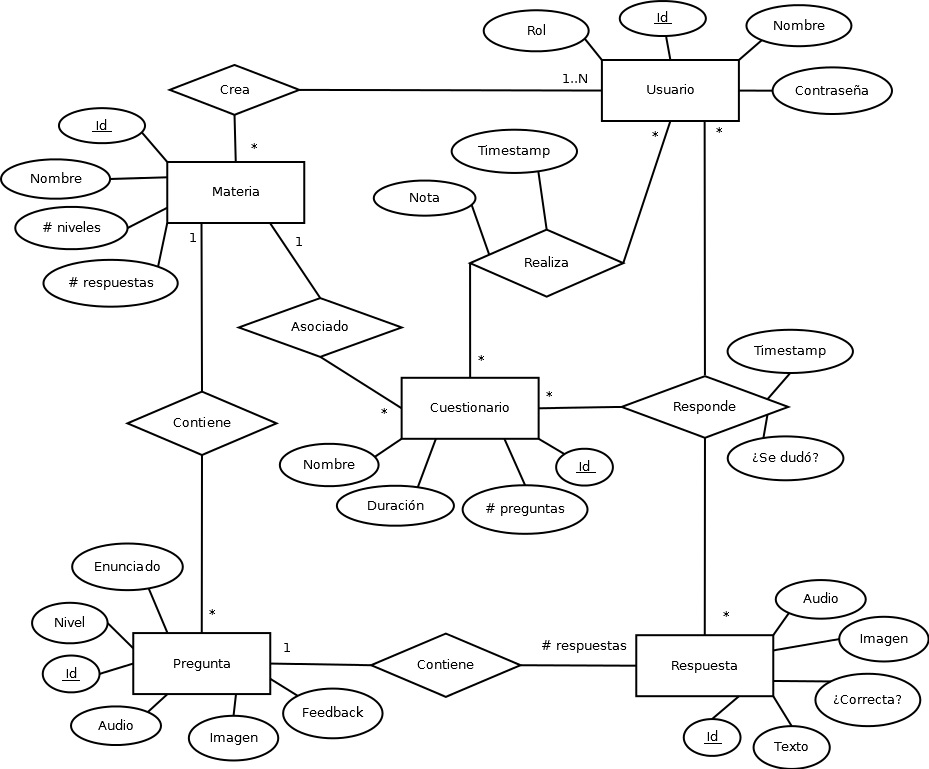
\includegraphics[width=1\textwidth]{diagrama_entidad_relacion}
	\caption{Diagrama entidad relación de la base de datos}
	\label{fig:base de datos}
\end{figure}

Buscando hacer la base de datos lo menos propensa a errores posible, se transformó el diagrama anterior a una 3NF. Para ello, se crearon tantas tablas como entidades aparecen en el diagrama, además de algunas tablas auxiliares. En concreto, se crearon dos tablas más, una para cada una de las relaciones N a N (usuario-materia, usuario-cuestionario) con las claves primarias (y los atributos de la relación, en el caso de usuario-cuestionario). 

Además, se creó una tabla para la relación triple entre usuario-cuestionario-respuesta. Esta relación recoge la información de cada respuesta que da cada alumno a cada pregunta que le aparece en cada cuestionario que realiza, guardando además el momento en el que se responde y si el alumno dudó al hacerlo. Aunque en un primer vistazo pueda parecer que existiendo esta relación sobra la relación entre usuario-cuestionario, ambas relaciones modelan información distinta. La relación usuario-cuestionario almacena el momento en el que un alumno empieza un cuestionario, y si lo termina, la nota que ha sacado en dicho intento, información independiente de cada una de las respuestas que vaya dando a lo largo del cuestionario, que es lo que guarda la relación triple.


\subsection{Módulos asociados al docente}

Las cuentas que dispongan de permisos de profesor pueden gestionar sus cuestionarios a través de la zona de profesor. Esta sección se divide en 4 módulos principales:

\begin{itemize}
	\item Gestión de Materias, Preguntas y Exámenes.
	\item Ficheros multimedia.
	\item Recuperación de exámenes.
	\item Análisis de resultados.
\end{itemize}

A continuación se repasarán las características y el funcionamiento de cada uno de ellos.

\subsubsection{Gestión de Materias, Preguntas y Exámenes}

Los módulos de materias, preguntas y exámenes son los encargados de permitir al usuario crear y gestionar las materias, preguntas y cuestionarios, respectivamente. Los tres tienen un funcionamiento muy parecido, similar al mostrado en la figura \ref{fig:e-valUAM interfaz profesor}.

\begin{figure}[htp!]
	\centering
	\includegraphics[width=1\textwidth,clip=true]{e-valUAM_preguntas}
	\caption{Interfaz de e-valUAM para el profesor}
	\label{fig:e-valUAM interfaz profesor}
\end{figure}

A través del menú superior, al docente puede acceder a todas las secciones de la página. Al entrar en ``Materias'', ``Preguntas'' o ``Exámenes'' verá una interfaz dividida en dos zonas. 

La zona primera (a la izquierda en la imagen, arriba si se accediera desde un dispositivo con una pantalla pequeña) es la que sirve para crear una nueva entidad en el sistema. Un formulario solicita al usuario toda la información relevante. Al pulsar en el botón de ``Guardar'', y tras comprobar con Javascript que todos los campos necesarios han sido rellenados, se envía al servidor. En el servidor un fichero PHP recibe la información, la valida y si todo es correcto, la almacena en la base de datos.

La segunda zona (a la derecha en la imagen, al final de la página se se accede con una pantalla pequeña) es donde se lista la información ya almacenada en la base de datos. En formato tabular se muestran todas las entradas. A la derecha del todo se muestran dos botones para editar la información y borrarla.

Cuando se edita un elemento, aparece un formulario en primer plano con la información almacenada hasta el momento y la posibilidad de establecer un nuevo valor para cada campo. Al final del formulario se ofrecen dos botones, para guardar los cambios o descartarlos sin alterar la base de datos. Un ejemplo es la figura \ref{fig:e-valUAM edicion profesor}.

\begin{figure}[htp!]
	\centering
	\includegraphics[width=0.75\textwidth,clip=true]{e-valUAM_edicion}
	\caption{Menú de edición para un elemento}
	\label{fig:e-valUAM edicion profesor}
\end{figure}

Si el usuario guarda los cambios, el navegador del usuario envía una petición AJAX con la información del cambio, que es comprobado y procesado por un fichero PHP en el servidor. El servidor responde si se ha podido realizar el cambio o no, para avisar al usuario en caso de que se produjera un error. Si se intenta borrar el elemento, el sistema pedirá confirmación y lanzará una petición AJAX al servidor siguiendo el mismo proceso.

\subsubsection{Ficheros multimedia}

Para poder trabajar con ficheros multimedia, la web permite a los docentes subir nuevos ficheros o listar los que ya estén. Los ficheros multimedia van asociados a una materia, así que lo primero que debe elegirse es con qué materia se quiere trabajar, tanto para ver como para listar, .

Para asegurar la compatibilidad con todos los navegadores modernos el sistema solo acepta imágenes en formatos GIF, PNG o JPEG y audio en formato MP3. Cuando el profesor sube un fichero se guarda en una carpeta en el servidor diferente para cada materia, por lo que cada profesor puede tener sus propios ficheros sin interferir con los demás. En la base de datos, mediante el gestor de preguntas, se asocian los ficheros con las preguntas y las respuestas. Cuando deben mostrarse al usuario, sencillamente el servidor busca el fichero en la carpeta correspondiente para que su navegador se lo muestre al usuario.

\begin{figure}[htp!]
	\centering
	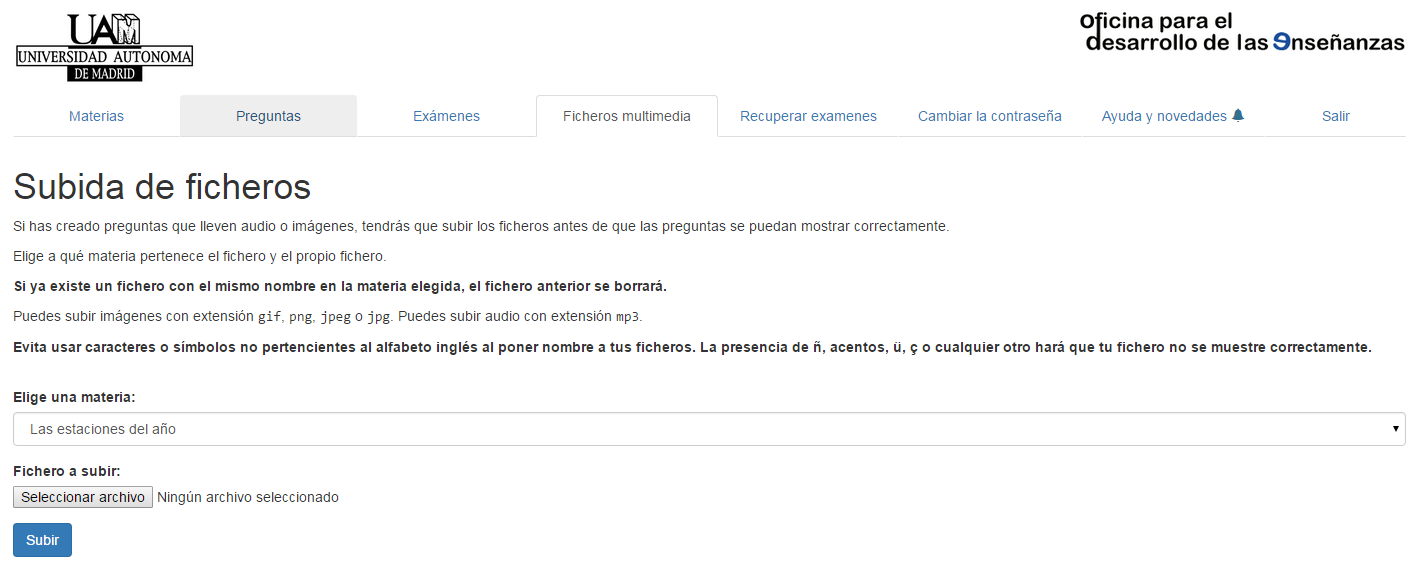
\includegraphics[width=0.75\textwidth,clip=true]{e-valUAM_multimedia}
	\caption{Subida de elementos multimedia}
	\label{fig:e-valUAM multimedia profesor}
\end{figure}

Para que el profesor no tenga que recordar qué ficheros subió o el nombre de los mismos, se incluyó la sección de visión de ficheros. Sencillamente, cuando el docente elige una materia para mostrar, se solicita por AJAX al servidor un listado de todos los ficheros que hay asociados a ella. Cuando el navegador recibe respuesta empieza a mostrarlos si son imágenes o a mostrar un reproductor si se trata de audio, como se muestra en la figura \ref{fig:e-valUAM visor multimedia profesor}.

\begin{figure}[htp!]
	\centering
	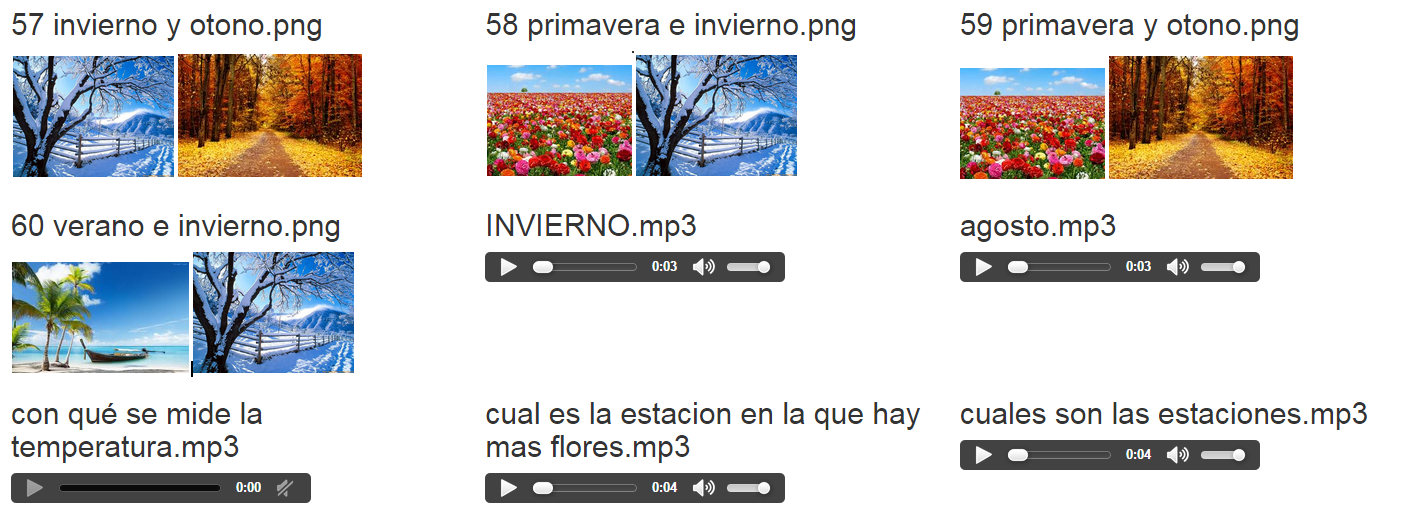
\includegraphics[width=0.75\textwidth,clip=true]{e-valUAM_visor_multimedia}
	\caption{Visor de elementos multimedia}
	\label{fig:e-valUAM visor multimedia profesor}
\end{figure}

\subsubsection{Recuperación de exámenes}

Aunque el sistema realiza una corrección automática de los cuestionarios respondidos por los alumnos, es posible que aún así los profesores deseen revisar los exámenes, ya sea para comprobar personalmente el desempeño de un alumno o para revisar con él sus respuestas o su calificación.

Con ese fin se creó el módulo de recuperación de exámenes. Cuando el profesor lo selecciona en el menú, aparece un listado con todos los cuestionarios que ha creado en algún momento. Cuando selecciona alguno de ellos, gracias a una petición AJAX, se muestra un listado con todos los intentos que ha realizado cada alumno respondiendo a ese cuestionario.

\begin{figure}[htp!]
	\centering
	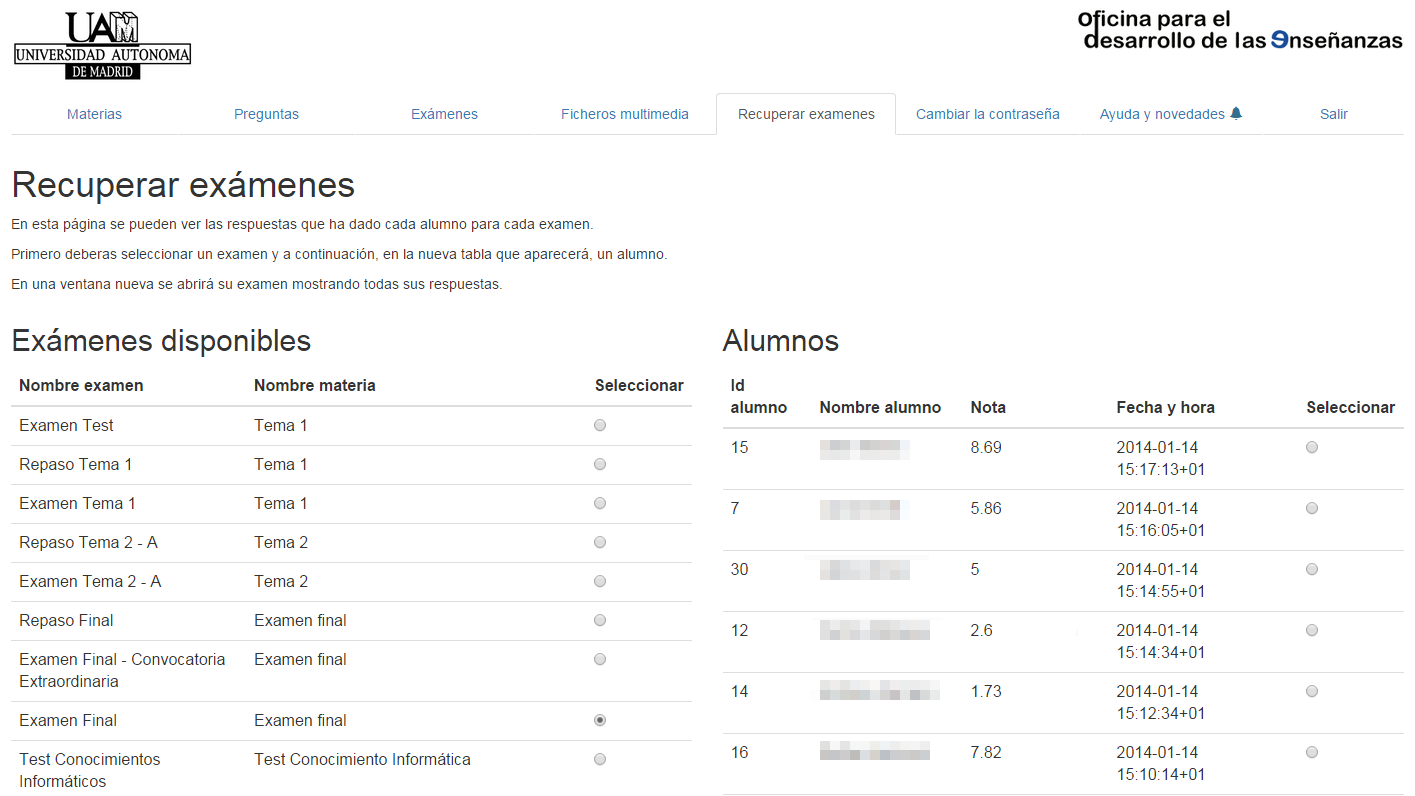
\includegraphics[width=1\textwidth,clip=true]{e-valUAM_recuperacion_examenes}
	\caption[Recuperación de exámenes]{Recuperación de exámenes. Se han difuminado el nombre de los alumnos por respeto a su intimidad.}
	\label{fig:e-valUAM recuperacion examenes profesor}
\end{figure}

Cuando el profesor selecciona un intento en concreto, el sistema muestra ordenadamente todas las preguntas que se eligieron para ese intento, junto a la respuesta que el alumno seleccionó, además de si esta es correcta o no. Para poder realizar esta operación correctamente es por lo que si un profesor modifica una pregunta no se borra de la base de datos, sino que se almacenan ambas versiones, de tal forma que siempre se recupera el examen tal y cómo lo vio el alumno en su momento.

\subsubsection{Análisis de resultados}

Una de las motivaciones de este trabajo es ayudar a los docentes en sus actividades automatizando aquellas que más tiempo les consuman. Desde esa perspectiva, un módulo de análisis de resultados es fundamental. En la versión actual, el módulo aún es muy primitivo ya que solo sirve para detectar preguntas con un ratio de fallo excesivo de forma automática. En un futuro se desean añadir más características a este módulo utilizando técnicas de machine learning.

Cuando el docente accede, tras seleccionar una materia y el número mínimo de veces que deben haber sido respondidas las preguntas para tenerse en cuenta, verá ordenadas todas las preguntas por el ratio de fallo. Aunque es un análisis todavía muy simple, permite quitar al profesor un gran trabajo, ya que revisar todos los cuestionarios manualmente, agrupando por preguntas y calculando ratio de fallos podría llevar horas, especialmente para grupos de alumnos grandes.

\subsection{Módulos asociados al estudiante}

Las secciones de la página destinas al estudiante son más sencillas y menos abundantes limitándose sencillamente a tres módulos que interaccionan siempre en un orden determinado. Cuando el alumno accede al sistema a través de la página principal, es redirigido a la página de elección de cuestionario, dónde se le ofrecen todos los cuestionarios disponibles para él en ese momento. Una vez que selecciona el cuestionario que desea realizar, este empieza.

\begin{figure}[!htp]
	\subfloat[Respuestas con texto e imagen\label{fig:e-valUAM examen}]{%
		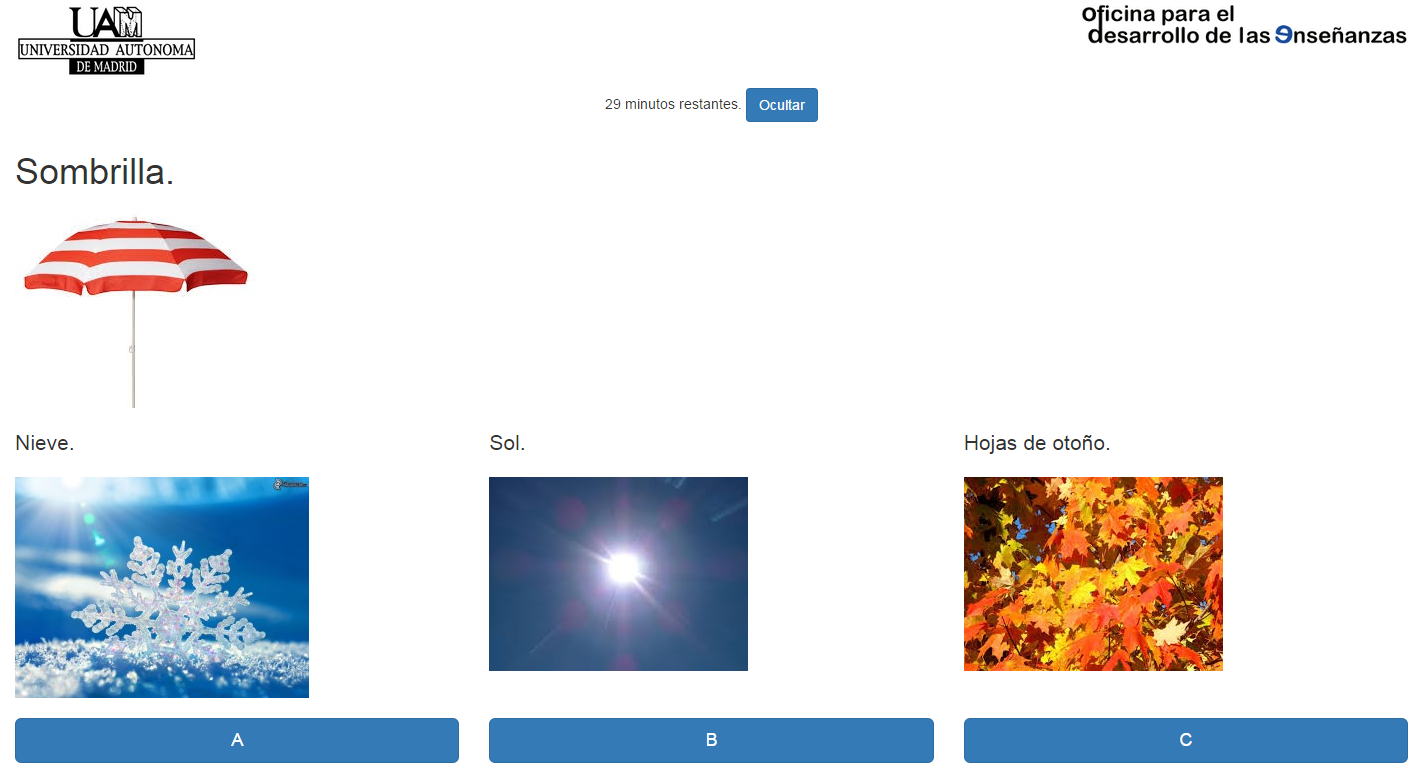
\includegraphics[width=0.45\textwidth]{e-valUAM_examen}
	}
	\hfill
	\subfloat[Respuestas con texto y audio\label{fig:e-valUAM examen audio}]{%
		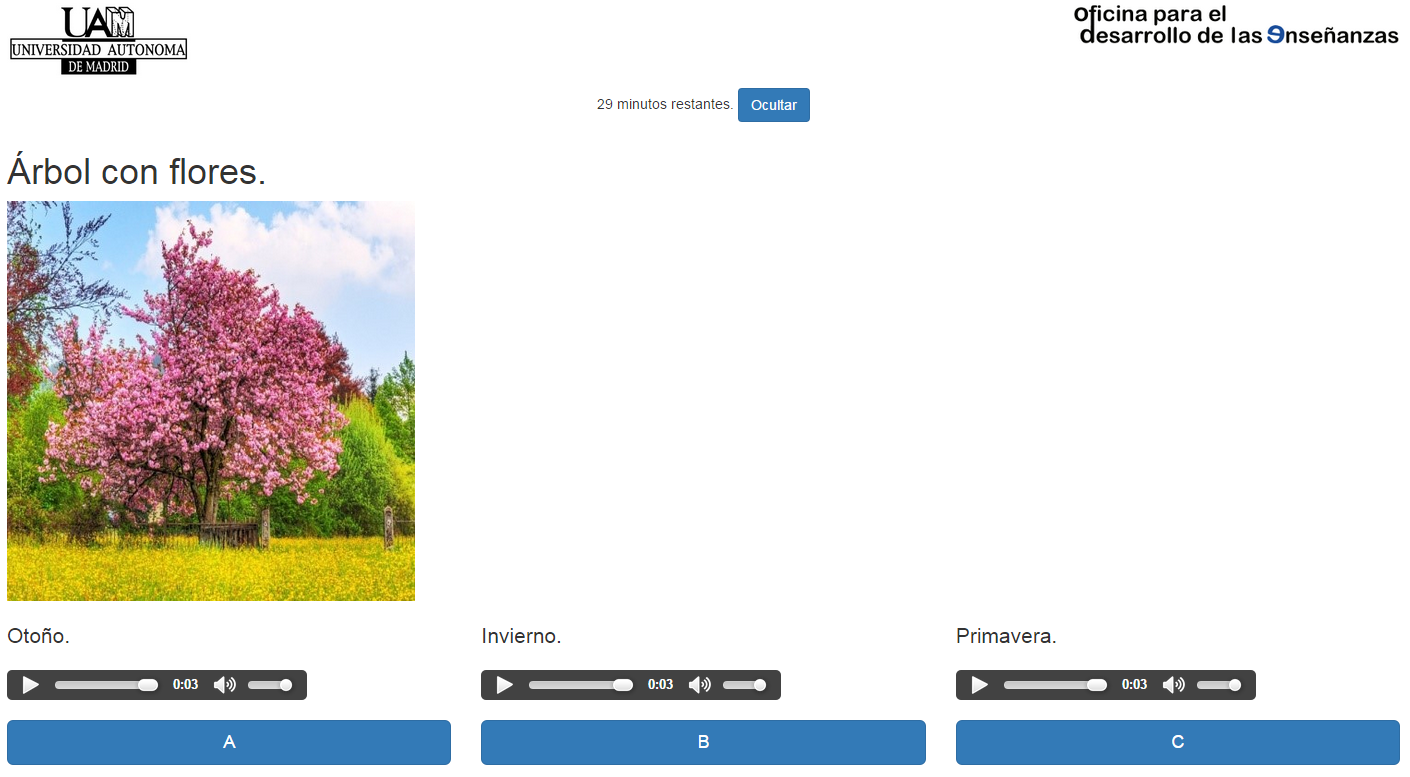
\includegraphics[width=0.45\textwidth]{e-valUAM_examen_audio}
	}
	\caption{Ejemplo de preguntas de un examen}
	\label{fig:e-valUAM examenes}
\end{figure}

Desde ese momento el sistema va seleccionando las preguntas siguiendo el modelo descrito en \ref{sec:modelo adapatacion}. Mientras al alumno aún le queden preguntas por responder y esté dentro del tiempo establecido por el profesor para responder, el examen continuará. Cuando termine con las preguntas o el tiempo, el cuestionario terminará. Dependiendo de qué opción haya elegido el profesor al fijar los parámetros el cuestionario, se mostrará un mensaje indicando que ha terminado el cuestionario, la nota o cada pregunta con la respuesta elegida estableciendo si ha sido correcta o no. A continuación el alumno puede abandonar el sistema o volver a probar con el mismo u otro cuestionario.

%\textbf{En la introducción dejar muy claro qué se ha desarrollado y qué no se ha desarrollado.}
